\documentclass{beamer}
\usepackage[T1]{fontenc}
\usepackage[utf8]{inputenc}
\usepackage{lmodern}

\title{Declutterization}
\author{Nathan Vance}
\date{}

\begin{document}

\begin{frame}
  \titlepage
\end{frame}

\begin{frame}
  \frametitle{Overview of the Declutterizer}
  \begin{enumerate}
    \item Generate cluttered images using the Clutterizer
    \item Train an SVM using clutter images
    \item Use the SVM to identify clutter in a novel clutter image
    \item Merge adjacent bounding boxes with the same label
  \end{enumerate}
\end{frame}

\begin{frame}
  \frametitle{Clutterization Process}
  \begin{enumerate}
    \item Images of individual objects were converted to PNGs with transparent backgrounds by hand.
    \item A scene is initialized to a random color.
    \item A random subset of objects are selected, resized, and rotated.
    \item The modified objects are added to the scene in a random order. The algorithm keeps track of their boundaries and occlusions.
    \item A labelme-formatted json file is written which corresponds to the generated clutter.
  \end{enumerate}
\end{frame}

\begin{frame}
  \frametitle{Clutterization Example}
  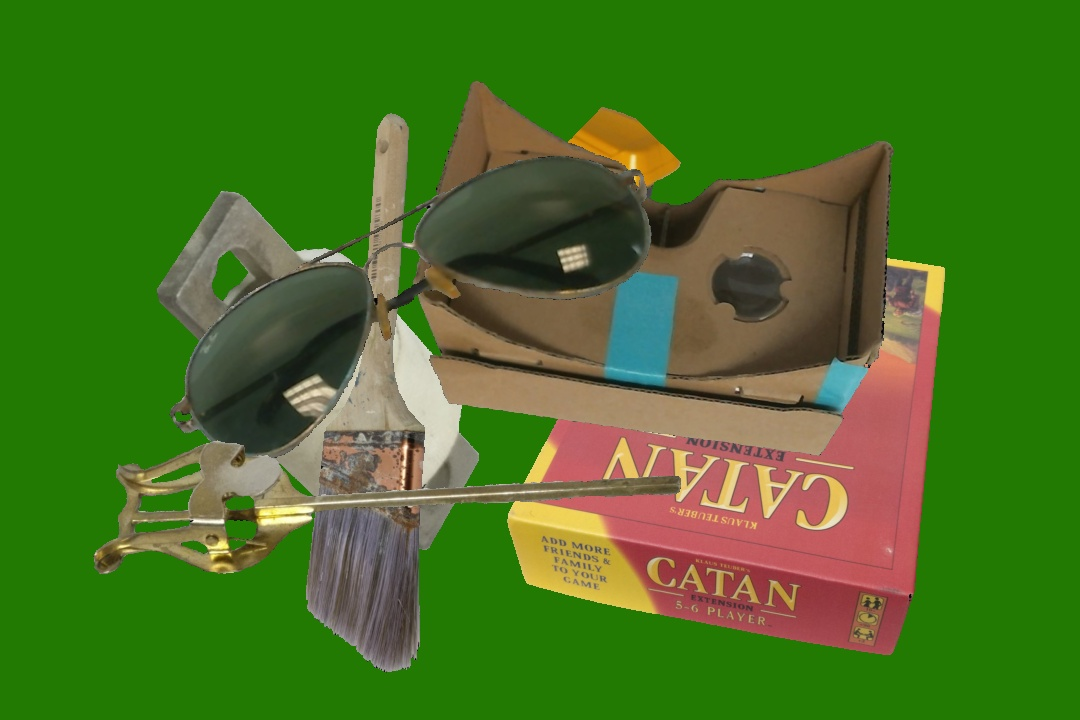
\includegraphics[width=\textwidth]{generated71.jpg}
\end{frame}

\begin{frame}
  \frametitle{Clutterization Example (cont)}
  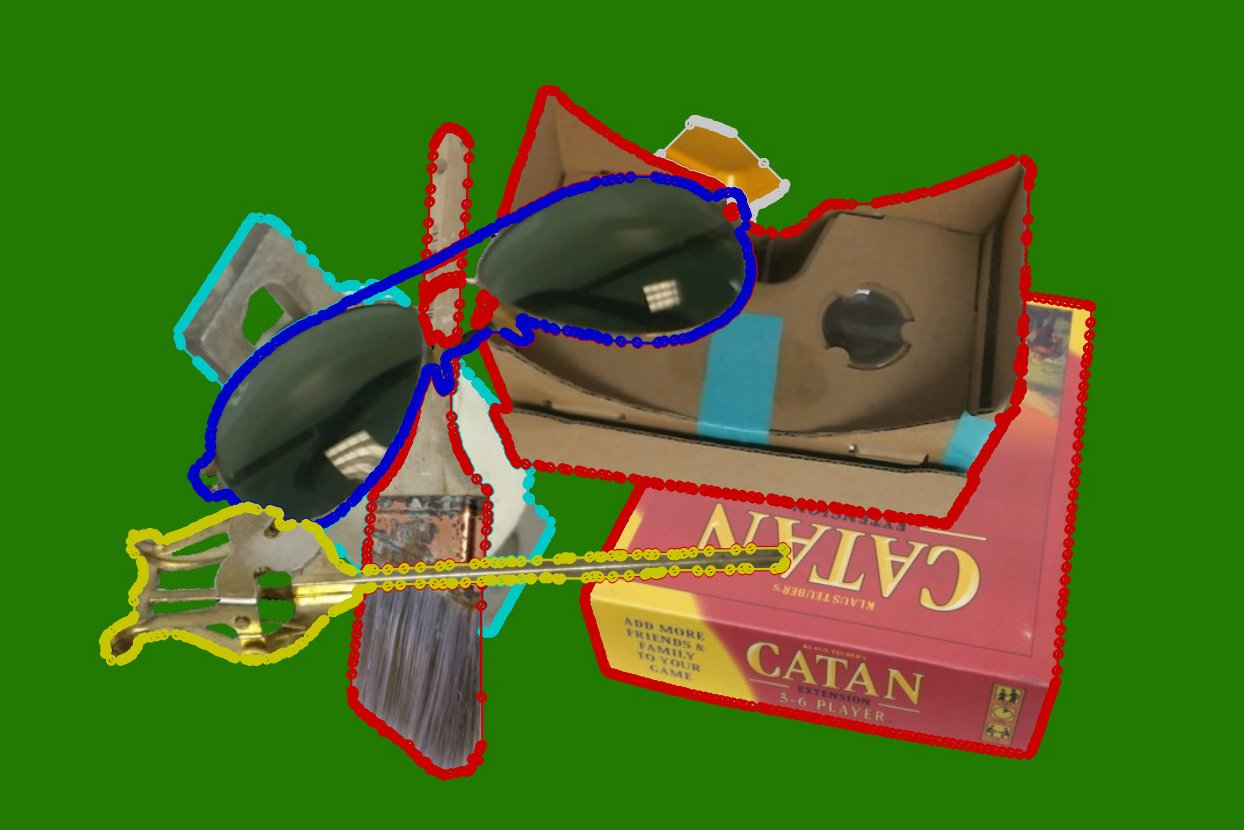
\includegraphics[width=\textwidth]{clutter.jpg}
\end{frame}

\begin{frame}
  \frametitle{Clutterization Example (cont)}
  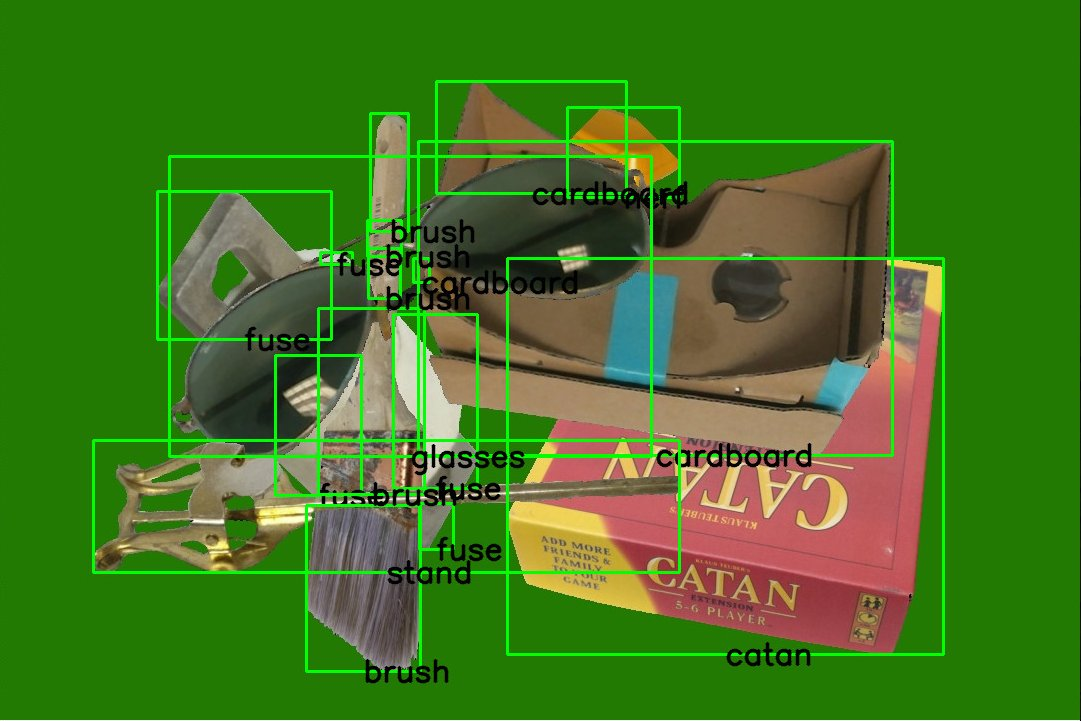
\includegraphics[width=\textwidth]{genTruth.jpg}
\end{frame}

\begin{frame}
  \frametitle{Feature Extraction}
  The following features are extracted:
  \begin{itemize}
    \item Normalized color histogram for the Hue channel in HSV colorspace
    \item Normalized LBP histograms for:
    \begin{itemize}
      \item 24 points at a radius of 8 pixels
      \item 16 points at a radius of 4 pixels
      \item 12 points at a radius of 2 pixels
      \item 8 points at a radius of 1 pixel (standard LBP)
    \end{itemize}
    \item Both feature spaces are rotation invariant.
  \end{itemize}
\end{frame}

\begin{frame}
  \frametitle{SVMs}
  Two models were employed in the solution:
  \begin{itemize}
    \item An SVM with an RBF kernel for classification (NuSVC in sklearn)
    \item A K-nearest-neighbors model for anomaly detection (LocalOutlierFactor in sklearn)
  \end{itemize}
\end{frame}

\begin{frame}
  \frametitle{Training}
  The models were trained using two different sources:
  \begin{itemize}
    \item The 92 images of the 10 objects that were converted to PNG, with backgrounds masked
    \item 70 clutterized images (generated from the PNG images)
  \end{itemize}
  In each case, the images were traversed with a sliding window. The system was then validated on 30 clutterized images.
\end{frame}

\begin{frame}
  \frametitle{Additional parameters}
  The following additional parameters were used:
  \begin{itemize}
    \item Sliding window size: 100x100 pixels
    \item Sliding window stride: 50 pixels
    \item Likelihood threshold to classify: 0.15
  \end{itemize}
\end{frame}

\begin{frame}
  \frametitle{Validation example}
  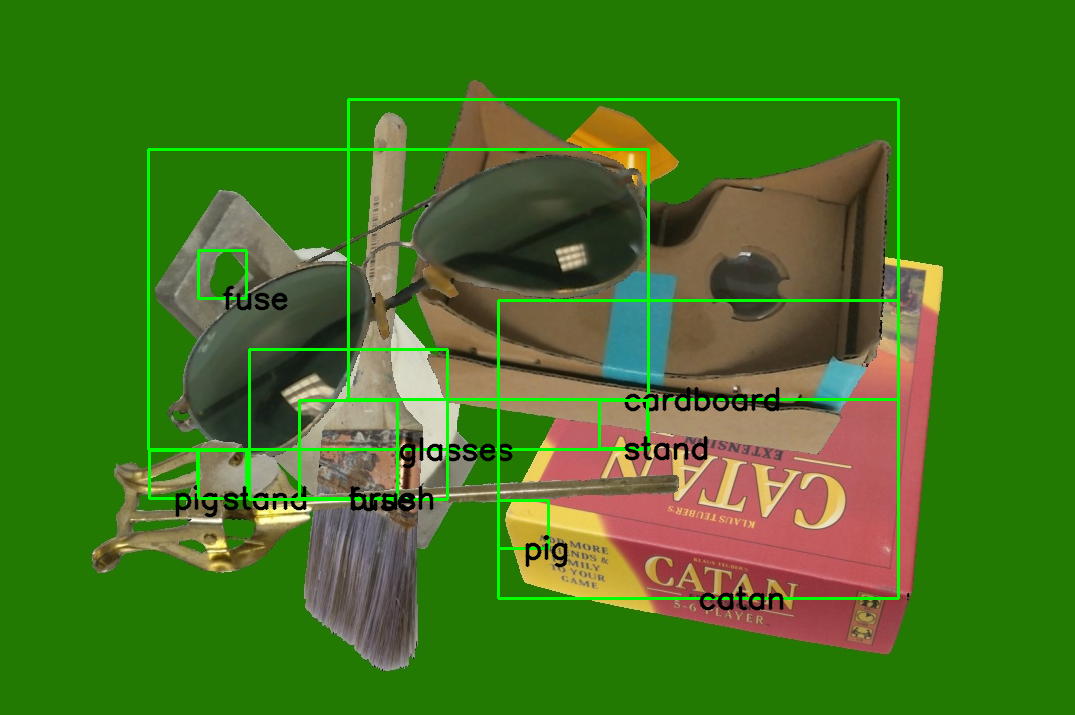
\includegraphics[width=\textwidth]{results.png}
\end{frame}

\begin{frame}
  \frametitle{Validation example (bad)}
  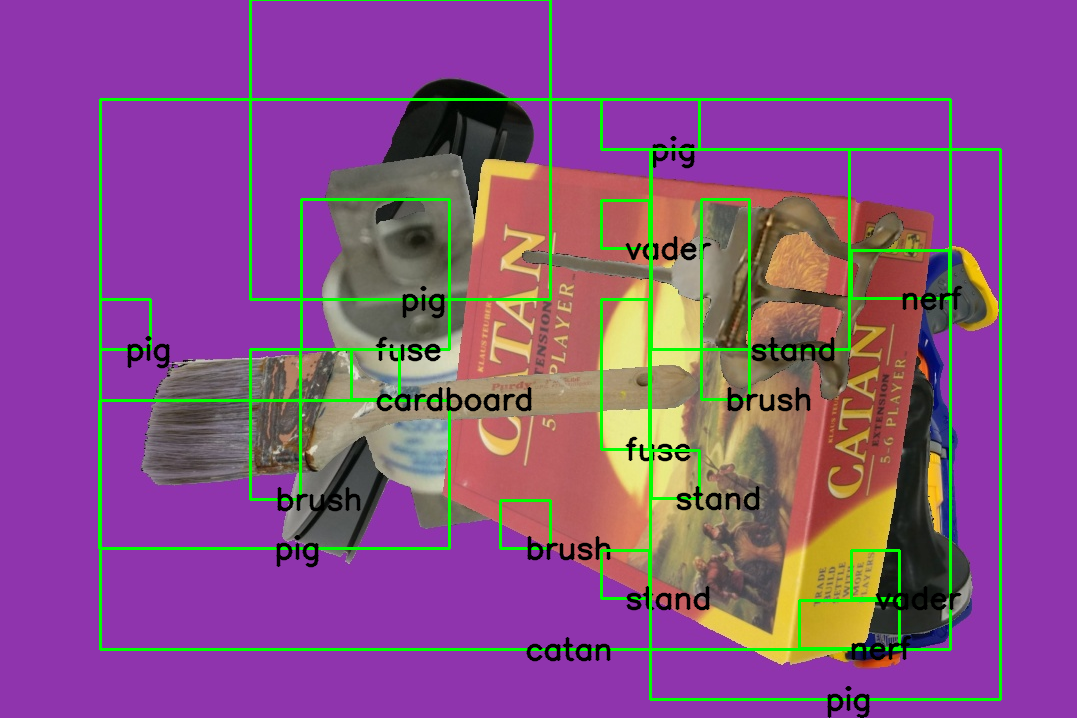
\includegraphics[width=\textwidth]{valResults2.png}
\end{frame}

\begin{frame}
  \frametitle{Validation results}
  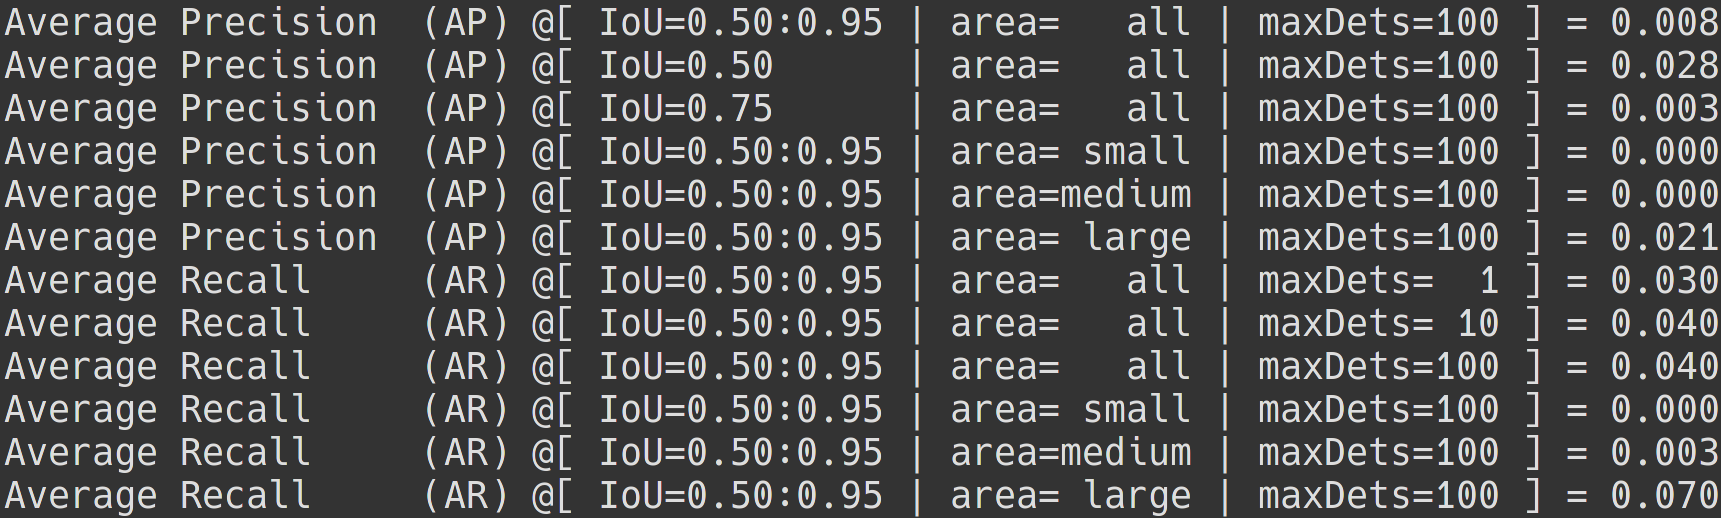
\includegraphics[width=\textwidth]{valScore.png}
\end{frame}

\begin{frame}
  \frametitle{Declutterization example}
  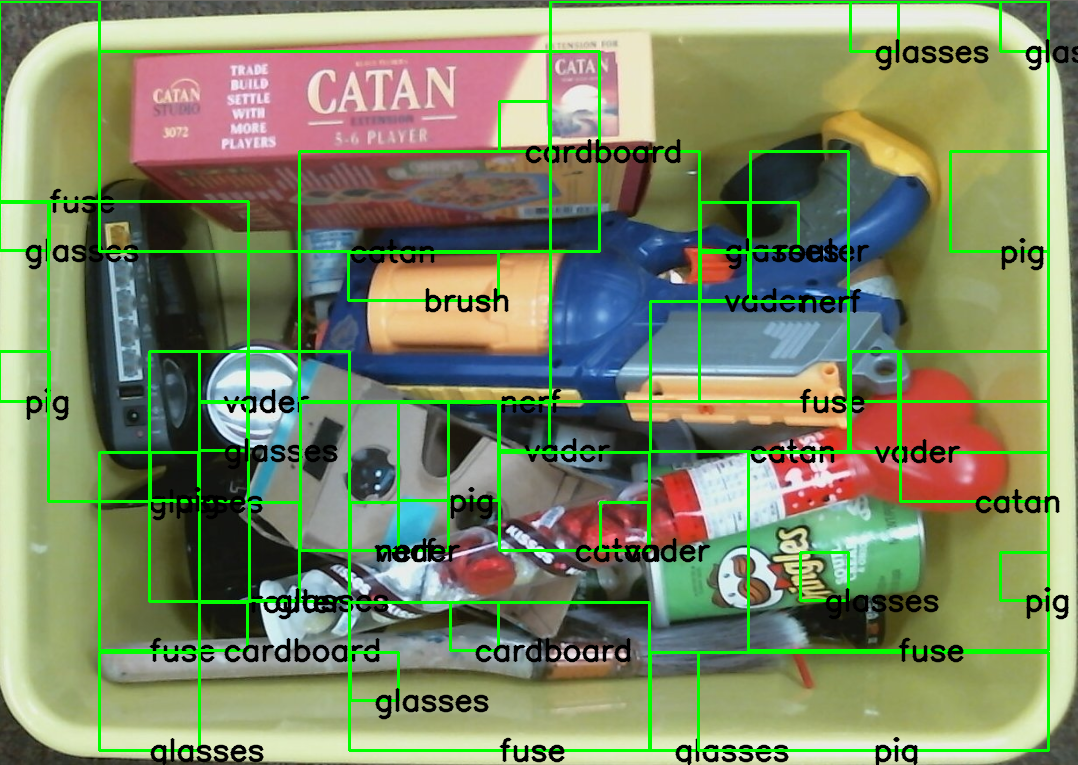
\includegraphics[width=\textwidth]{testResults.png}
\end{frame}

\begin{frame}
  \frametitle{Declutterization example (bad)}
  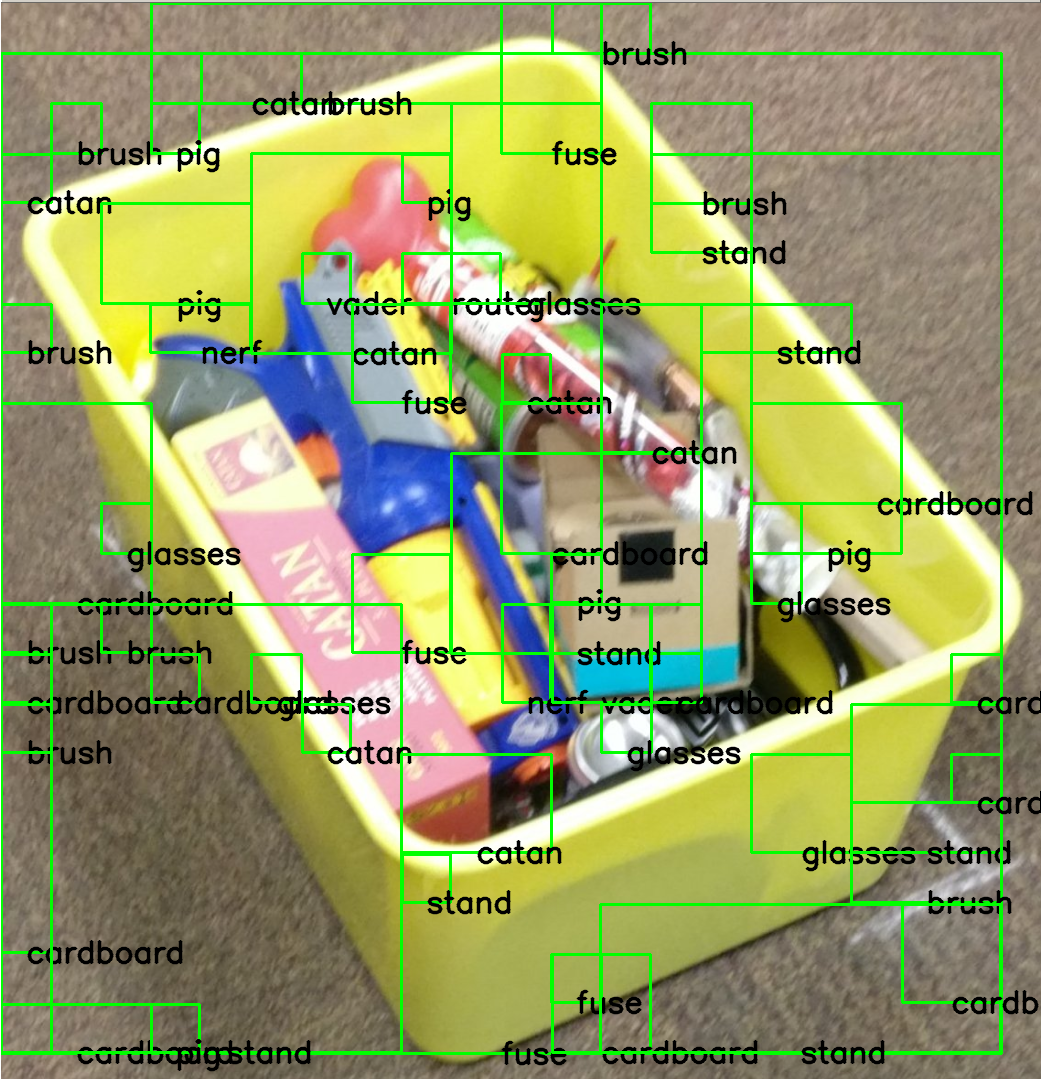
\includegraphics[height=.7\textwidth]{testResults2.png}
\end{frame}

\begin{frame}
  \frametitle{Declutterization results}
  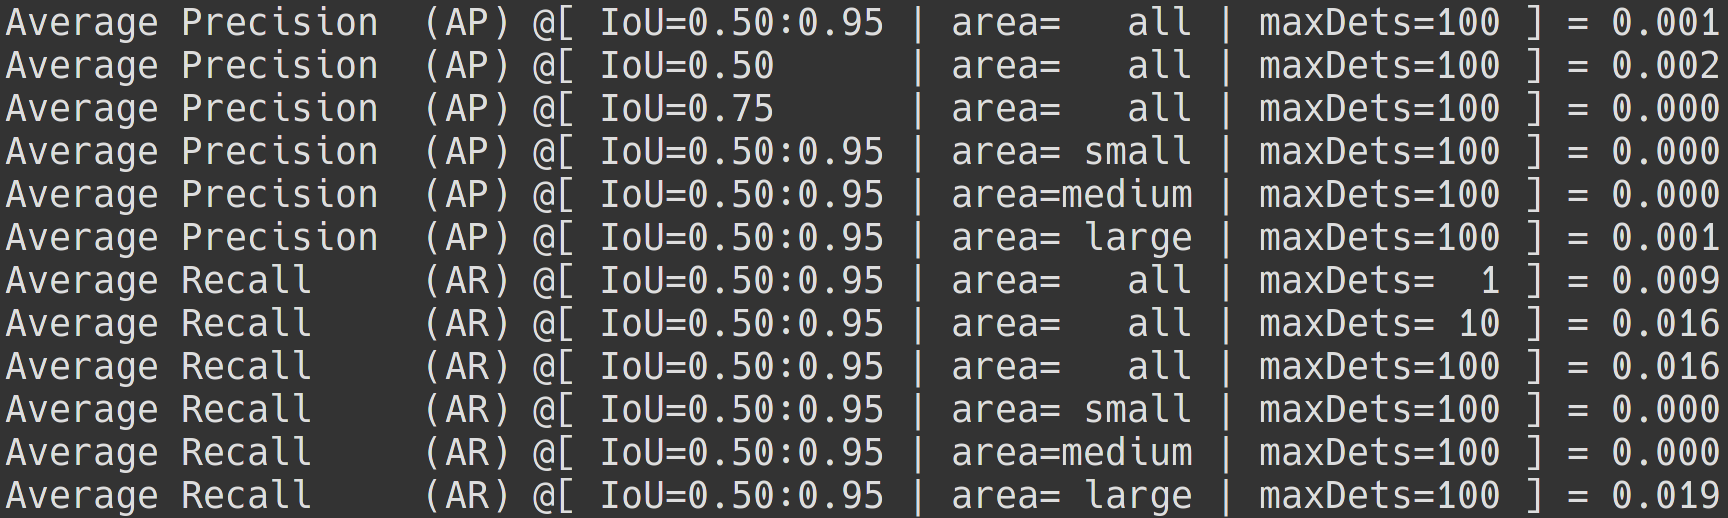
\includegraphics[width=\textwidth]{testScore.png}
\end{frame}

\begin{frame}
  \frametitle{Unknown input}
  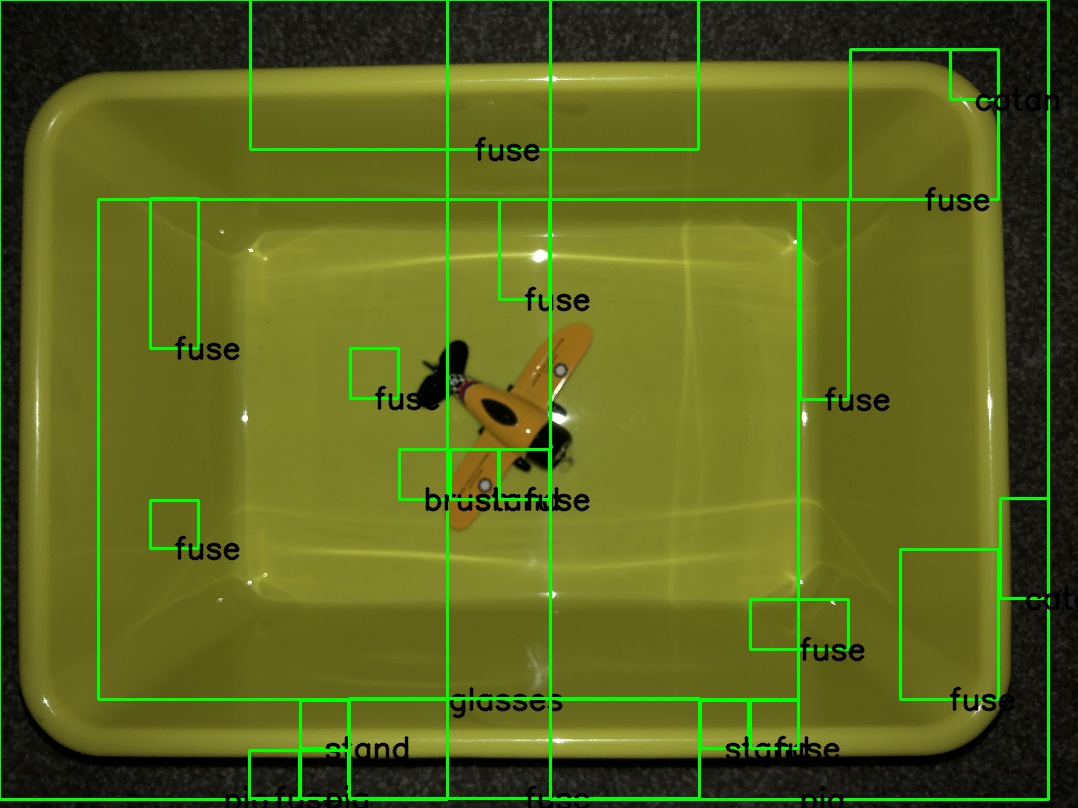
\includegraphics[width=\textwidth]{unknown1.png}
\end{frame}

\begin{frame}
  \frametitle{Unknown input}
  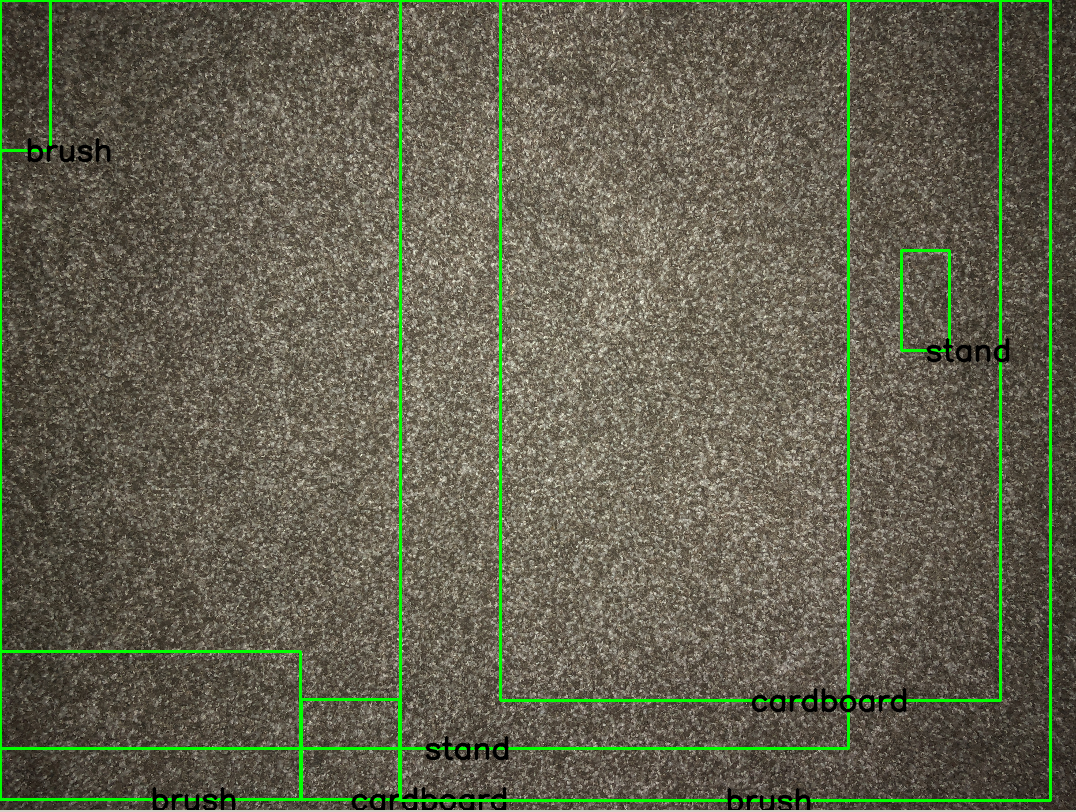
\includegraphics[width=\textwidth]{unknown2.png}
\end{frame}

\begin{frame}
  \frametitle{Unknown input}
  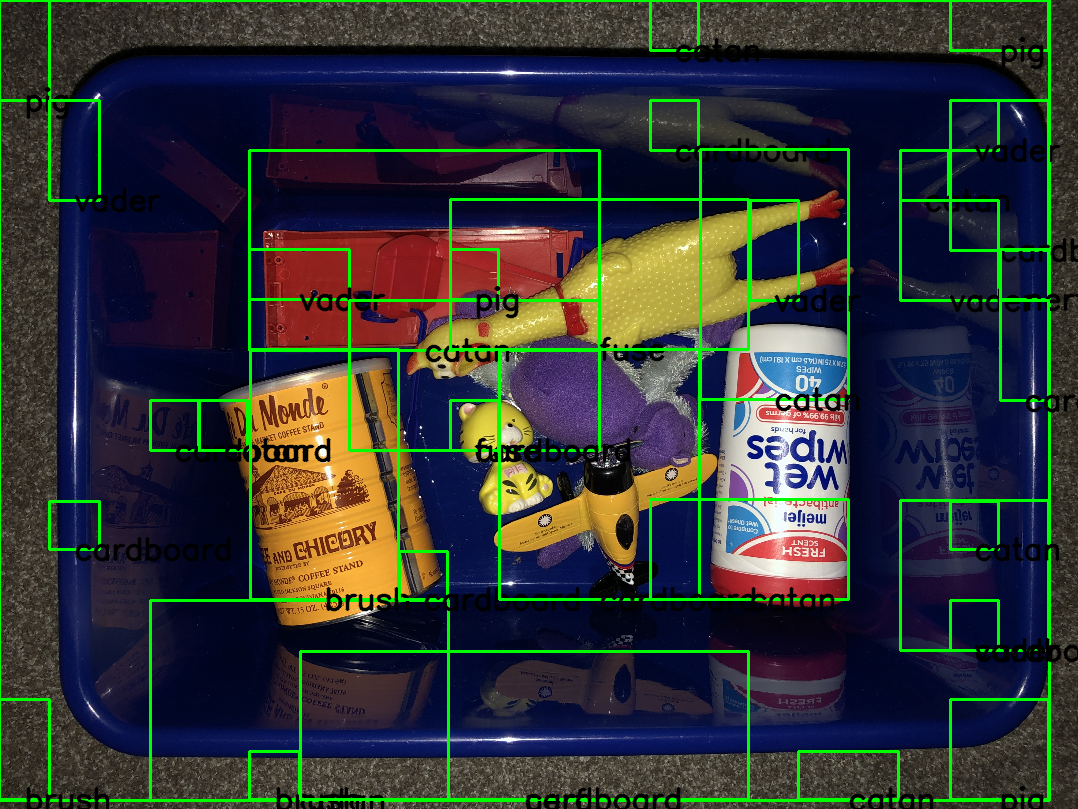
\includegraphics[width=\textwidth]{unknown3.png}
\end{frame}

\begin{frame}
  \frametitle{Conclusions}
  \begin{itemize}
    \item Qualitatively, the system does provide useful results.
    \item Using the official COCO scoring method, the system looks really bad.
    \item When tested on the unknown input, the system produces many false-positives.
  \end{itemize}
\end{frame}

\end{document}
